\section{Machine and Controller Design and Validation}
    \subsection{Current Controller Design}
        The current controller is designed based on two aspects: the converter and the AC synchronous generator.
        \subsubsection{Converter Design}
            A buck converter was used to convert a relatively high input voltage (\(V_{in}\)) to a lower field voltage (\(V_{f}\)). Although the topology of the buck converter was provided, a corresponding transfer function was derived to improve the simulation speed. Nonetheless, the optimal values of inductance and capacitance of the converter had to be calculated for the provided simscape model and the transfer function. 
            
            Assuming resistances in the buck converter are minimal and using the field resistance (\(R_f\)) and inductance (\(L_f\)) as the converters load, the following equation can be used to work out the values of inductance (\(L\)) and capacitance (\(C_{out}\)) in the converter:

            \begin{align}
                L = \frac{V_{out}\times(V_{in} - V_{out})}{\Delta I_L \times f_{sw} \times V_{in}} = 1.04 \times 10^{-4} \text{H} && C_{out} = \frac{\Delta I_L}{8 \times f_{sw} \times \Delta V_{out}} = 3 \times 10^{-4} \text{C},
            \end{align}
            where \(\Delta I_L\) and \(\Delta V_{out}\) are the current and voltage ripple.

            These values were used in the simscape model and derived transfer function producing the response to changes in duty cycle in Figure \ref{fig: converter output}. The response confirmed that the transfer function was viable, with little steady-state error, and although it doesn't account for transient effects, these are under a short time duration.
            \begin{figure}[tbh!]
                \centering
                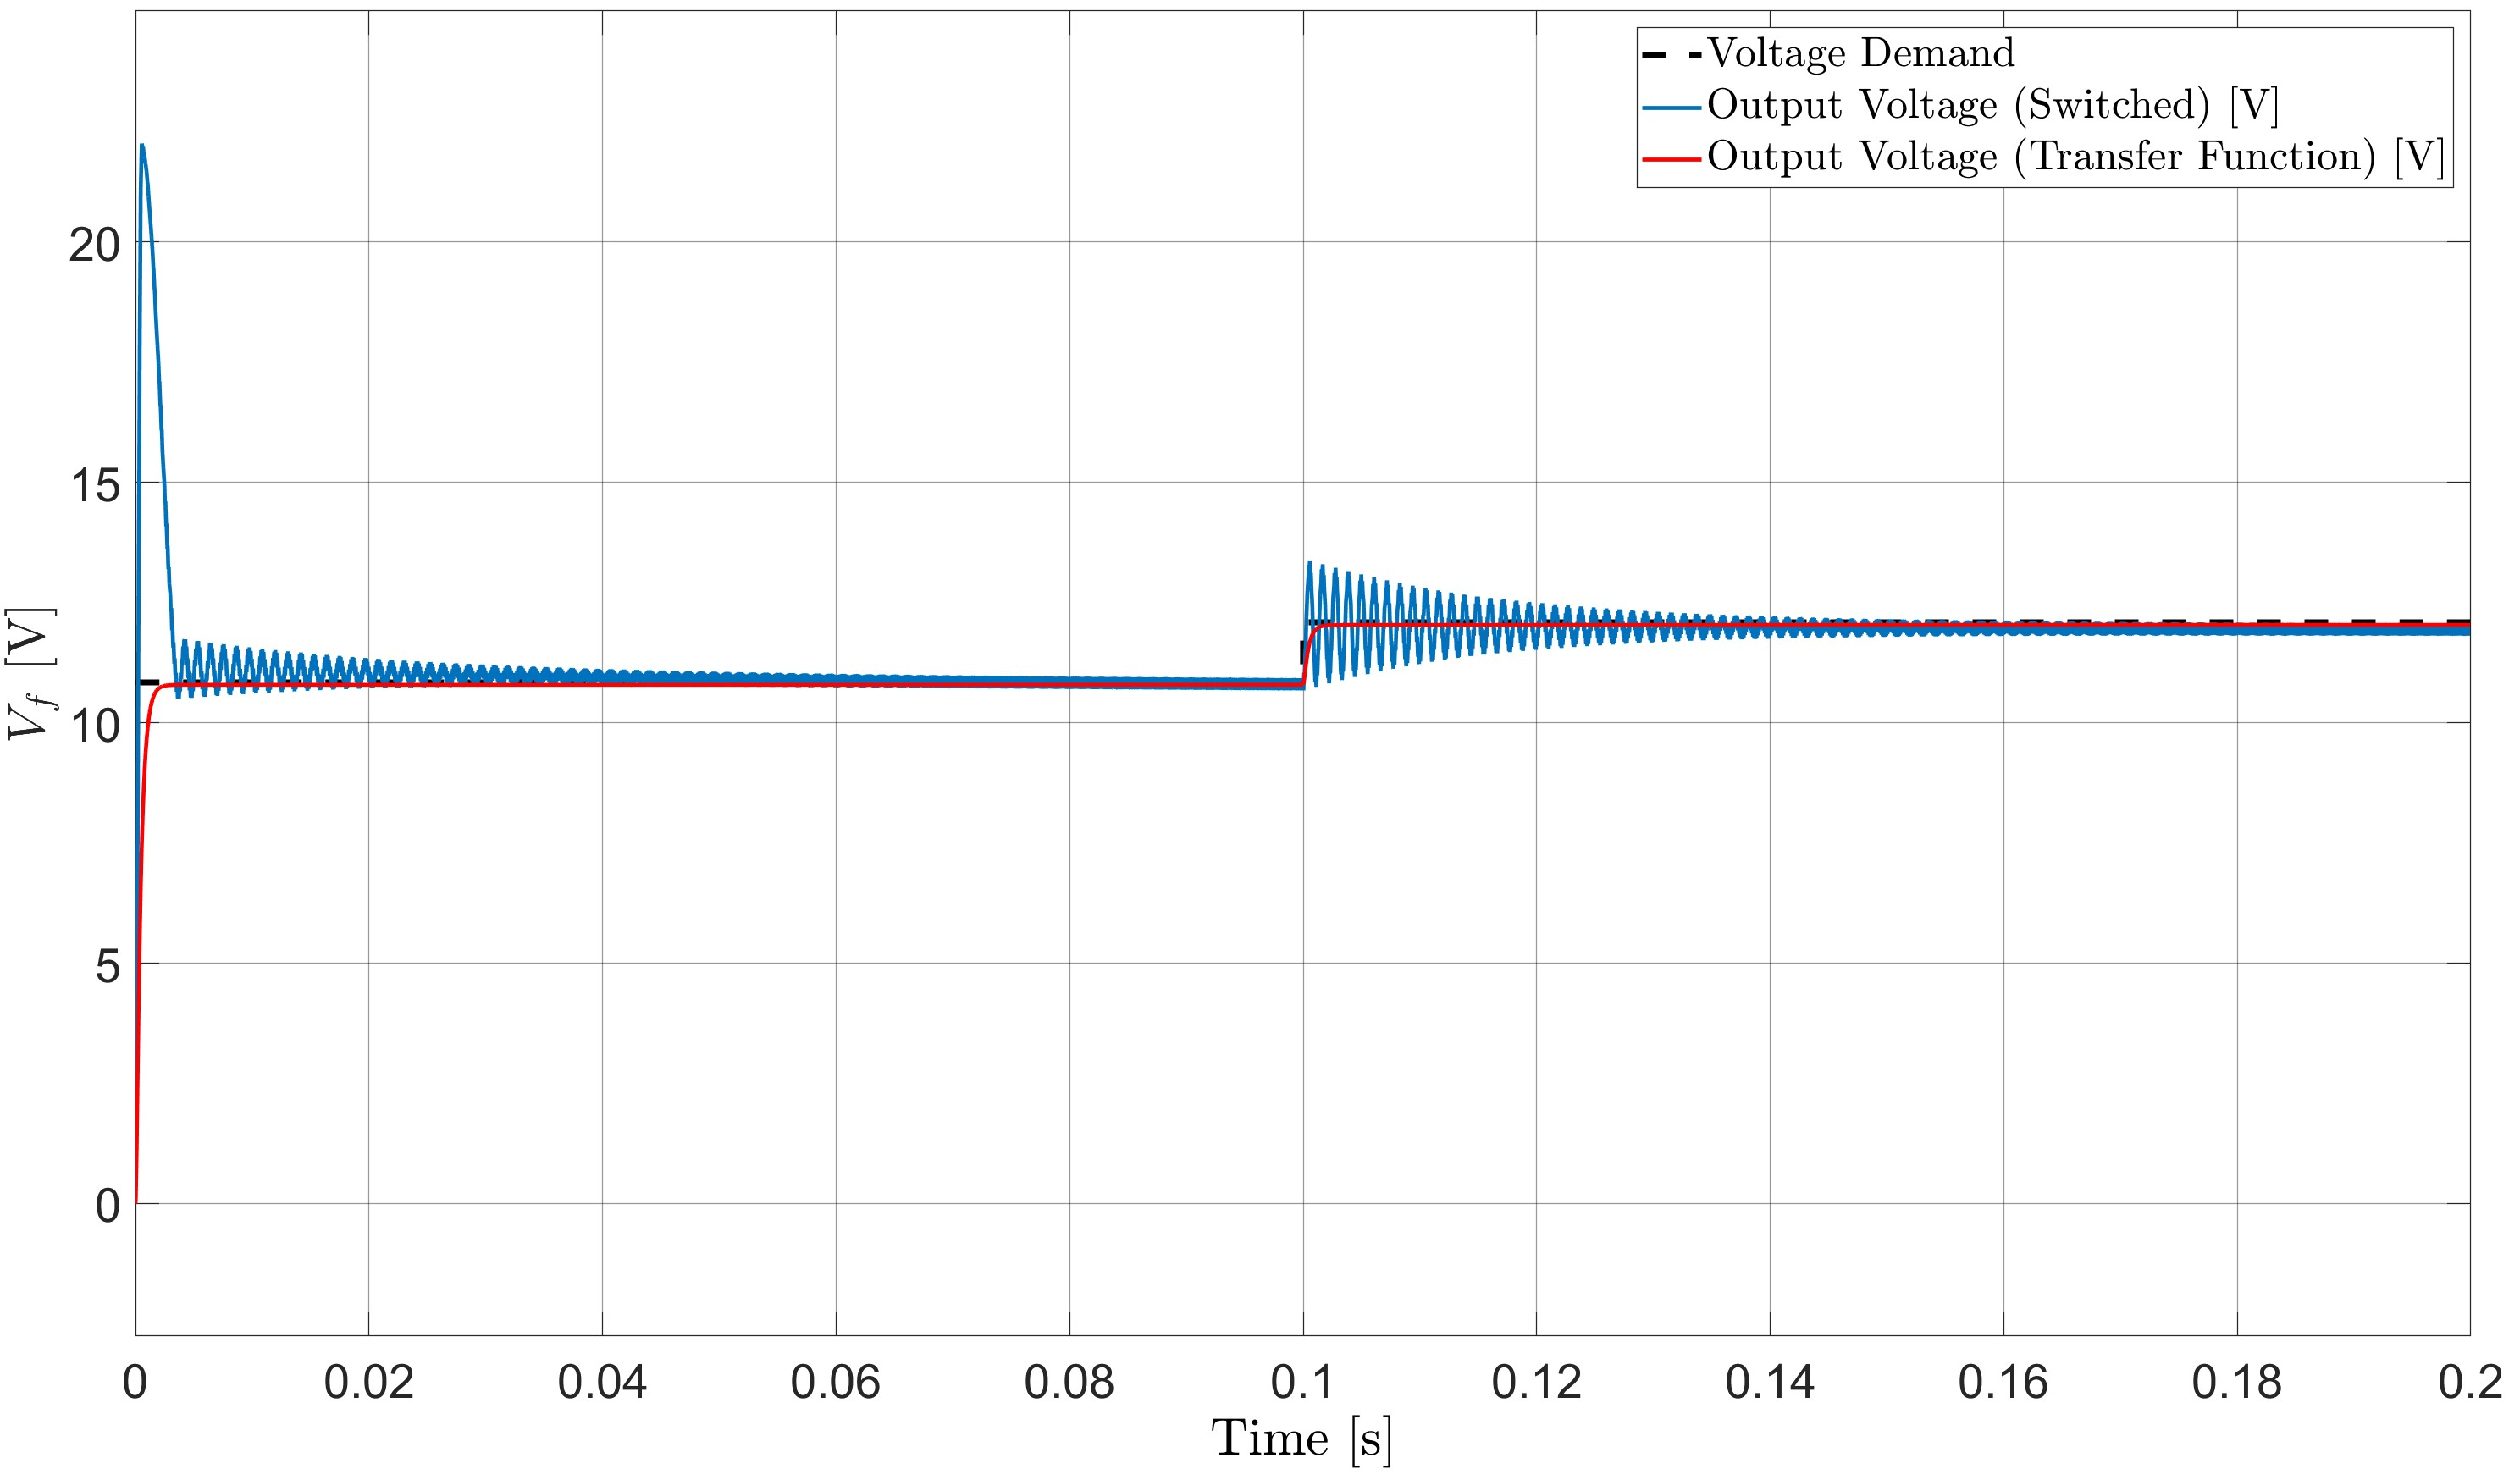
\includegraphics[width=0.5\linewidth]{PEMDT Exam Report/img/ConverterResponse.jpg}
                \caption{Comparison of desired voltage output, simscape model and transfer function of the buck converter}
                \label{fig: converter output}
            \end{figure}

        \subsubsection{Proportional + Integral Current Controller Design}
            To design the current controller for the wound field of the machine, three components in the system had to be taken into account. The first component was the AC machine. It was assumed that the machine acts like a wound field of a DC machine. Under this assumption, the following equivalent transfer function for the AC synchronous generator was formed:
            \begin{equation}
                G_{machine} = \frac{I_f(s)}{V_f(s)} = \frac{\frac{1}{L_f}}{s+\frac{R_f}{L_f}},
            \end{equation}
            where \(L_f\) and \(R_f\) are the field's inductance and resistance respectively. 

            The other component in the system is the P+I controller, which was set up using the following transfer function:
            \begin{equation}
                G_{controller} = K_p + \frac{K_i}{s},
            \end{equation}
            where \(K_p\) and \(K_i\) are the proportional and integral gains of the controller.

            The final component was the converter. Using the transfer function derived for the converter, it was found that the input and output of the converter had a linear relationship in steady state, as shown in Figure \ref{fig: converter grad}. Therefore, in the transfer loop, the converter was assumed to be a fixed value of \(Converter_{const.} = 25\) (the gradient of the line relating input to output).
            \begin{figure}
                \centering
                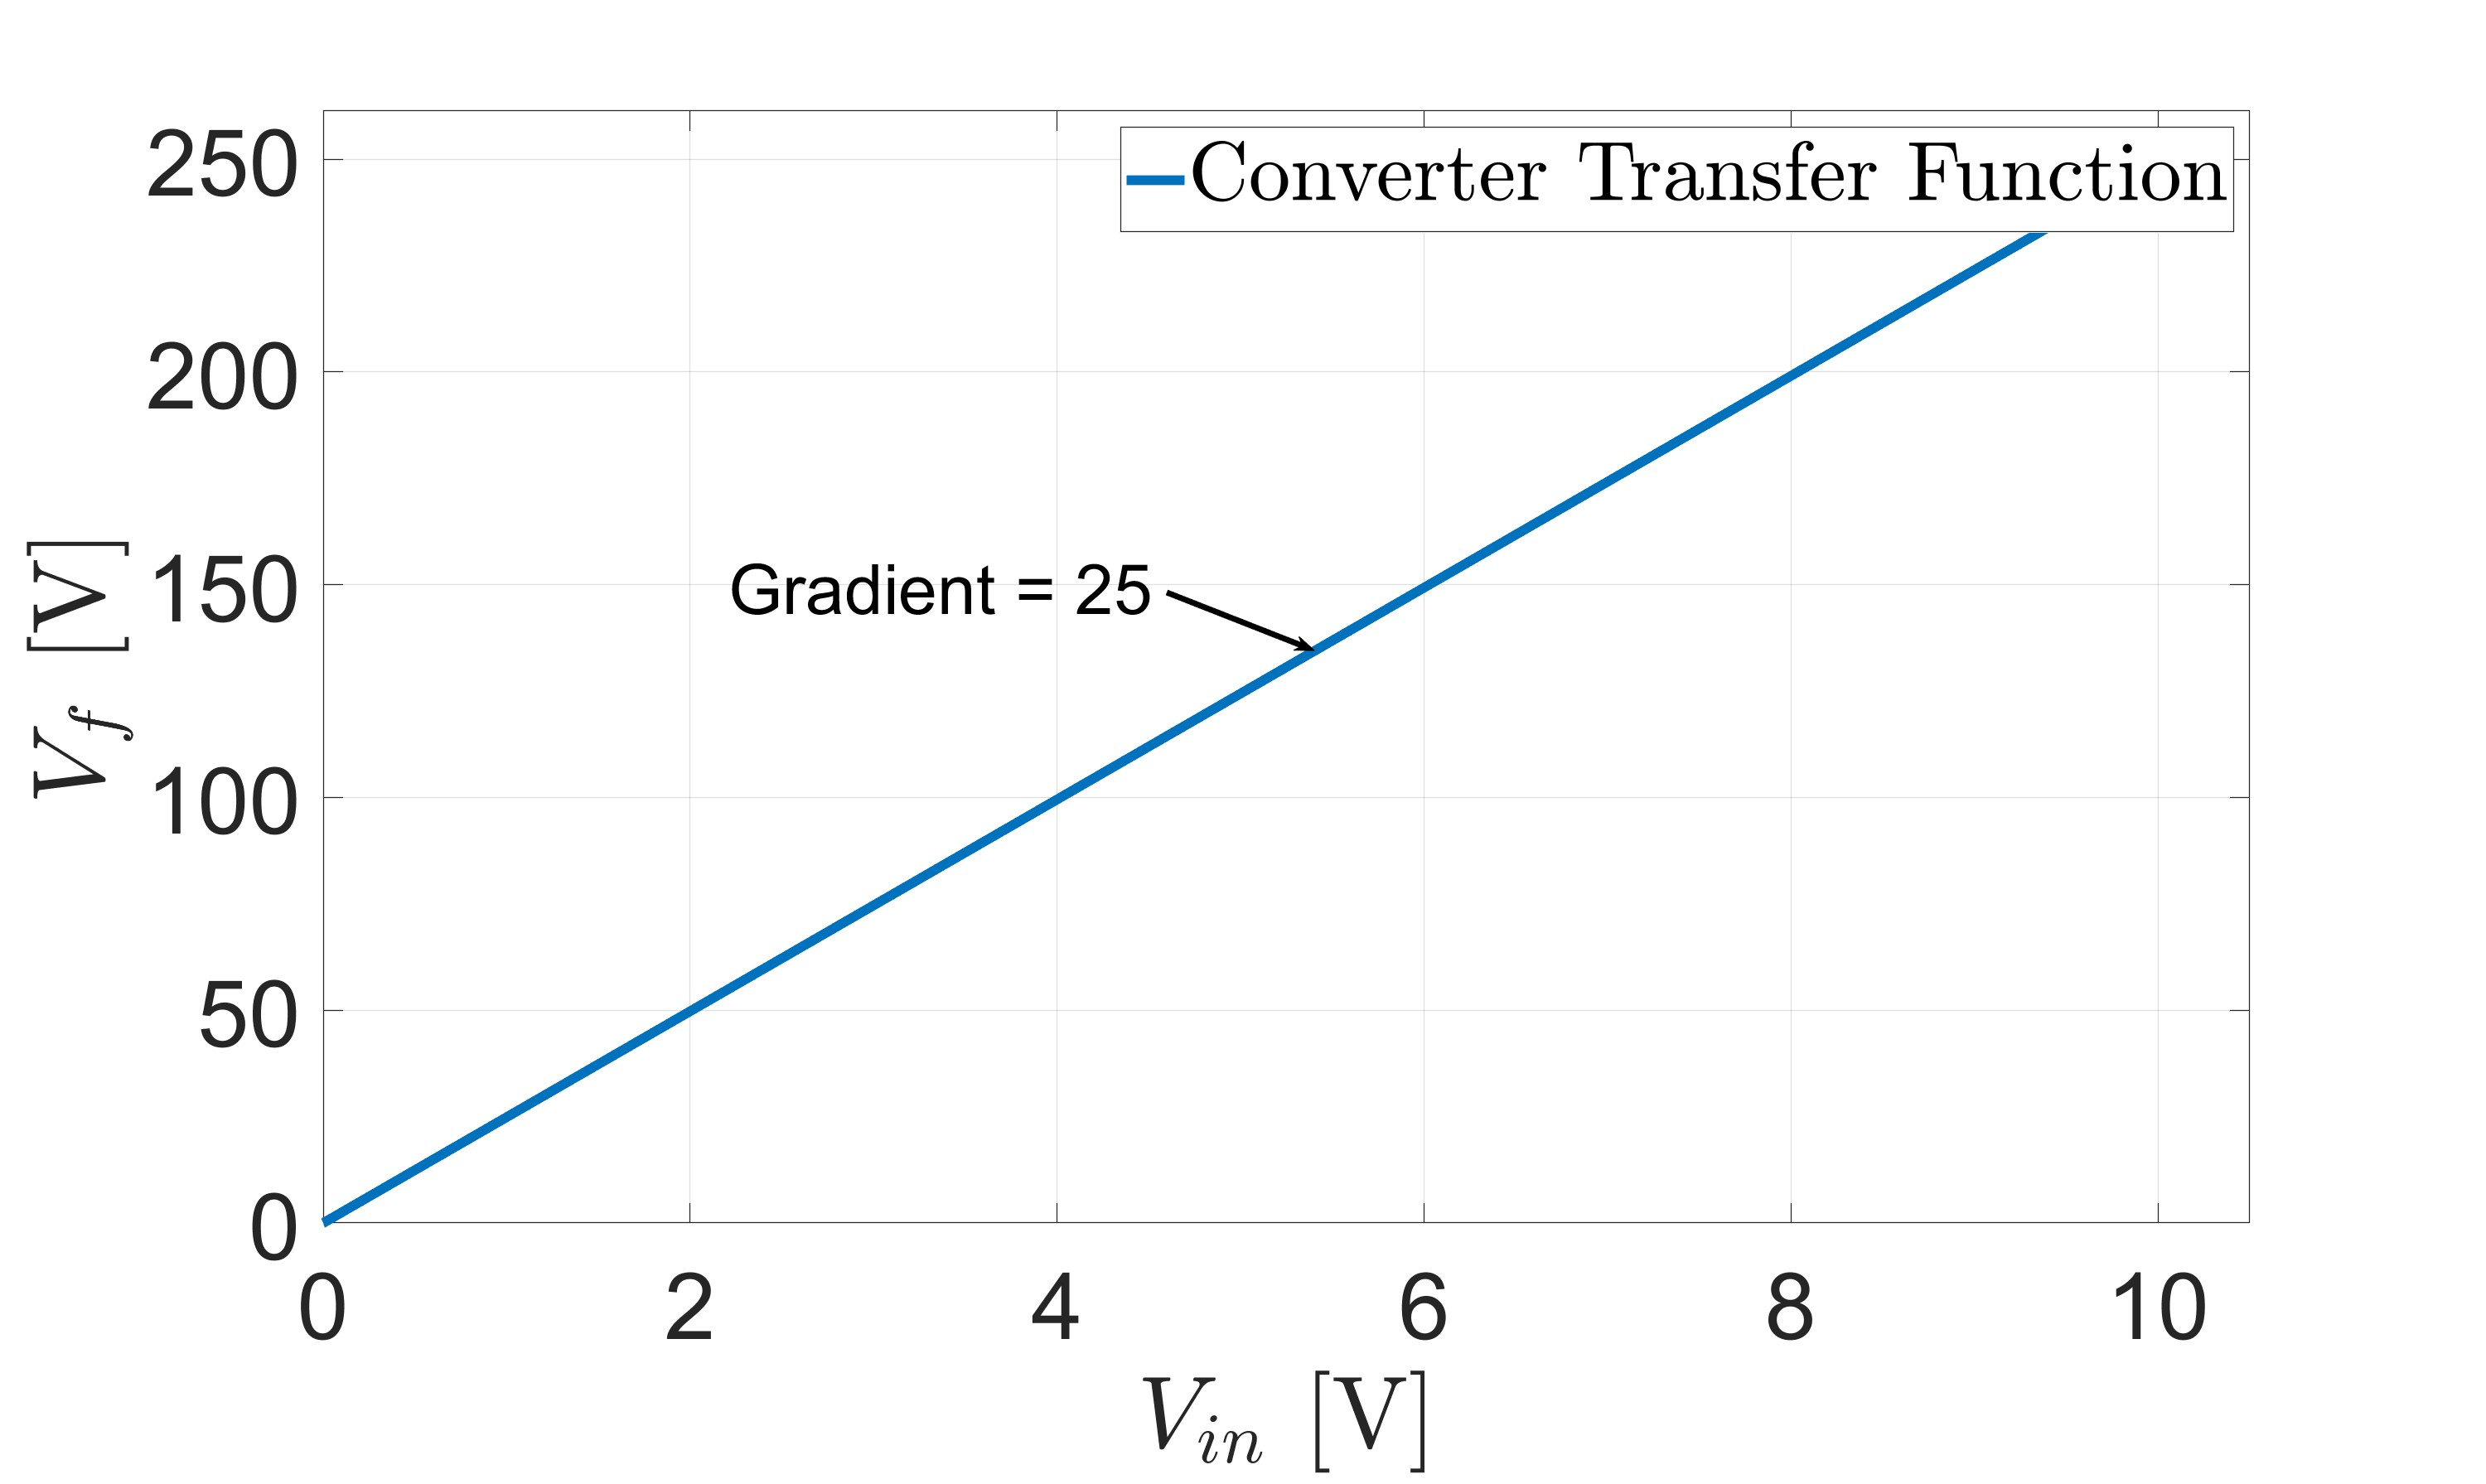
\includegraphics[width=0.5\linewidth]{PEMDT Exam Report/img/gradientconverter.jpg}
                \caption{Constant gradient between input and output of converter}
                \label{fig: converter grad}
            \end{figure}

            This all gave a final feedback transfer function as follows:
            \begin{equation}
                \frac{I_f(s)}{I_{ref}(s)} = \frac{G_{controller}G_{converter}G_{machine}}{1+G_{controller}G_{converter}G_{machine}} = \frac{\left(s+\frac{K_i}{K_p}\right)\frac{K_p \cdot R_f \cdot Converter_{const}}{L_f}}{s^2+s\left(\frac{L_f}{R_f} + K_p\frac{R_f \cdot Converter_{const}}{L_f}\right) + K_i\frac{R_f \cdot Converter_{const}}{L_f}} \label{eqn: character eqn}
            \end{equation}

            By setting \(K_p\) and \(K_i\) in the characteristic equation on the denominator of Eq. (\ref{eqn: character eqn}), there is complete control over the system's response. However, these values have to be calculated to place the poles in the correct position. Given the system should have a suitably fast and non-oscillatory response, the characteristic equation was compared to the ideal characteristic equation for a critically damped system, which for a second-order system is given by:
            \begin{equation}
                G_{ideal}(s) = \left(\frac{\frac{\lambda}{T}}{s+\left(\frac{1}{T}\right)}\right)^2 = \frac{\left(\frac{\lambda}{T}\right)^2}{s^2+\frac{2}{T}s + \frac{1}{T^2}}, \label{ideal sys}
            \end{equation}
            where \(T\) is the time period and is roughly a fifth of the settling time \(T = \frac{t_s}{5}\).

            Since a fast response is wanted, a settling time \(t_s = 0.2\)s was used. This provided an ideal closed-loop characteristic equation which was compared to the feedback characteristic equation:
            \begin{equation}
                s^2 + 50s + 625 = s^2+s\left(\frac{L_f}{R_f} + K_p\frac{R_f \cdot Converter_{const}}{L_f}\right) + K_i\frac{R_f \cdot Converter_{const}}{L_f},
            \end{equation}
            which showed that \(K_p = 0.124\) and \(K_i = 1.547\).

            This transfer function was set up with these values, and the response is shown in Figure \ref{fig: current resp}. Although it has an overshoot, it doesn't go above the max. current, it isn't oscillating and settles in roughly 0.5s.
            \begin{figure}[tbh!]
            \centering
            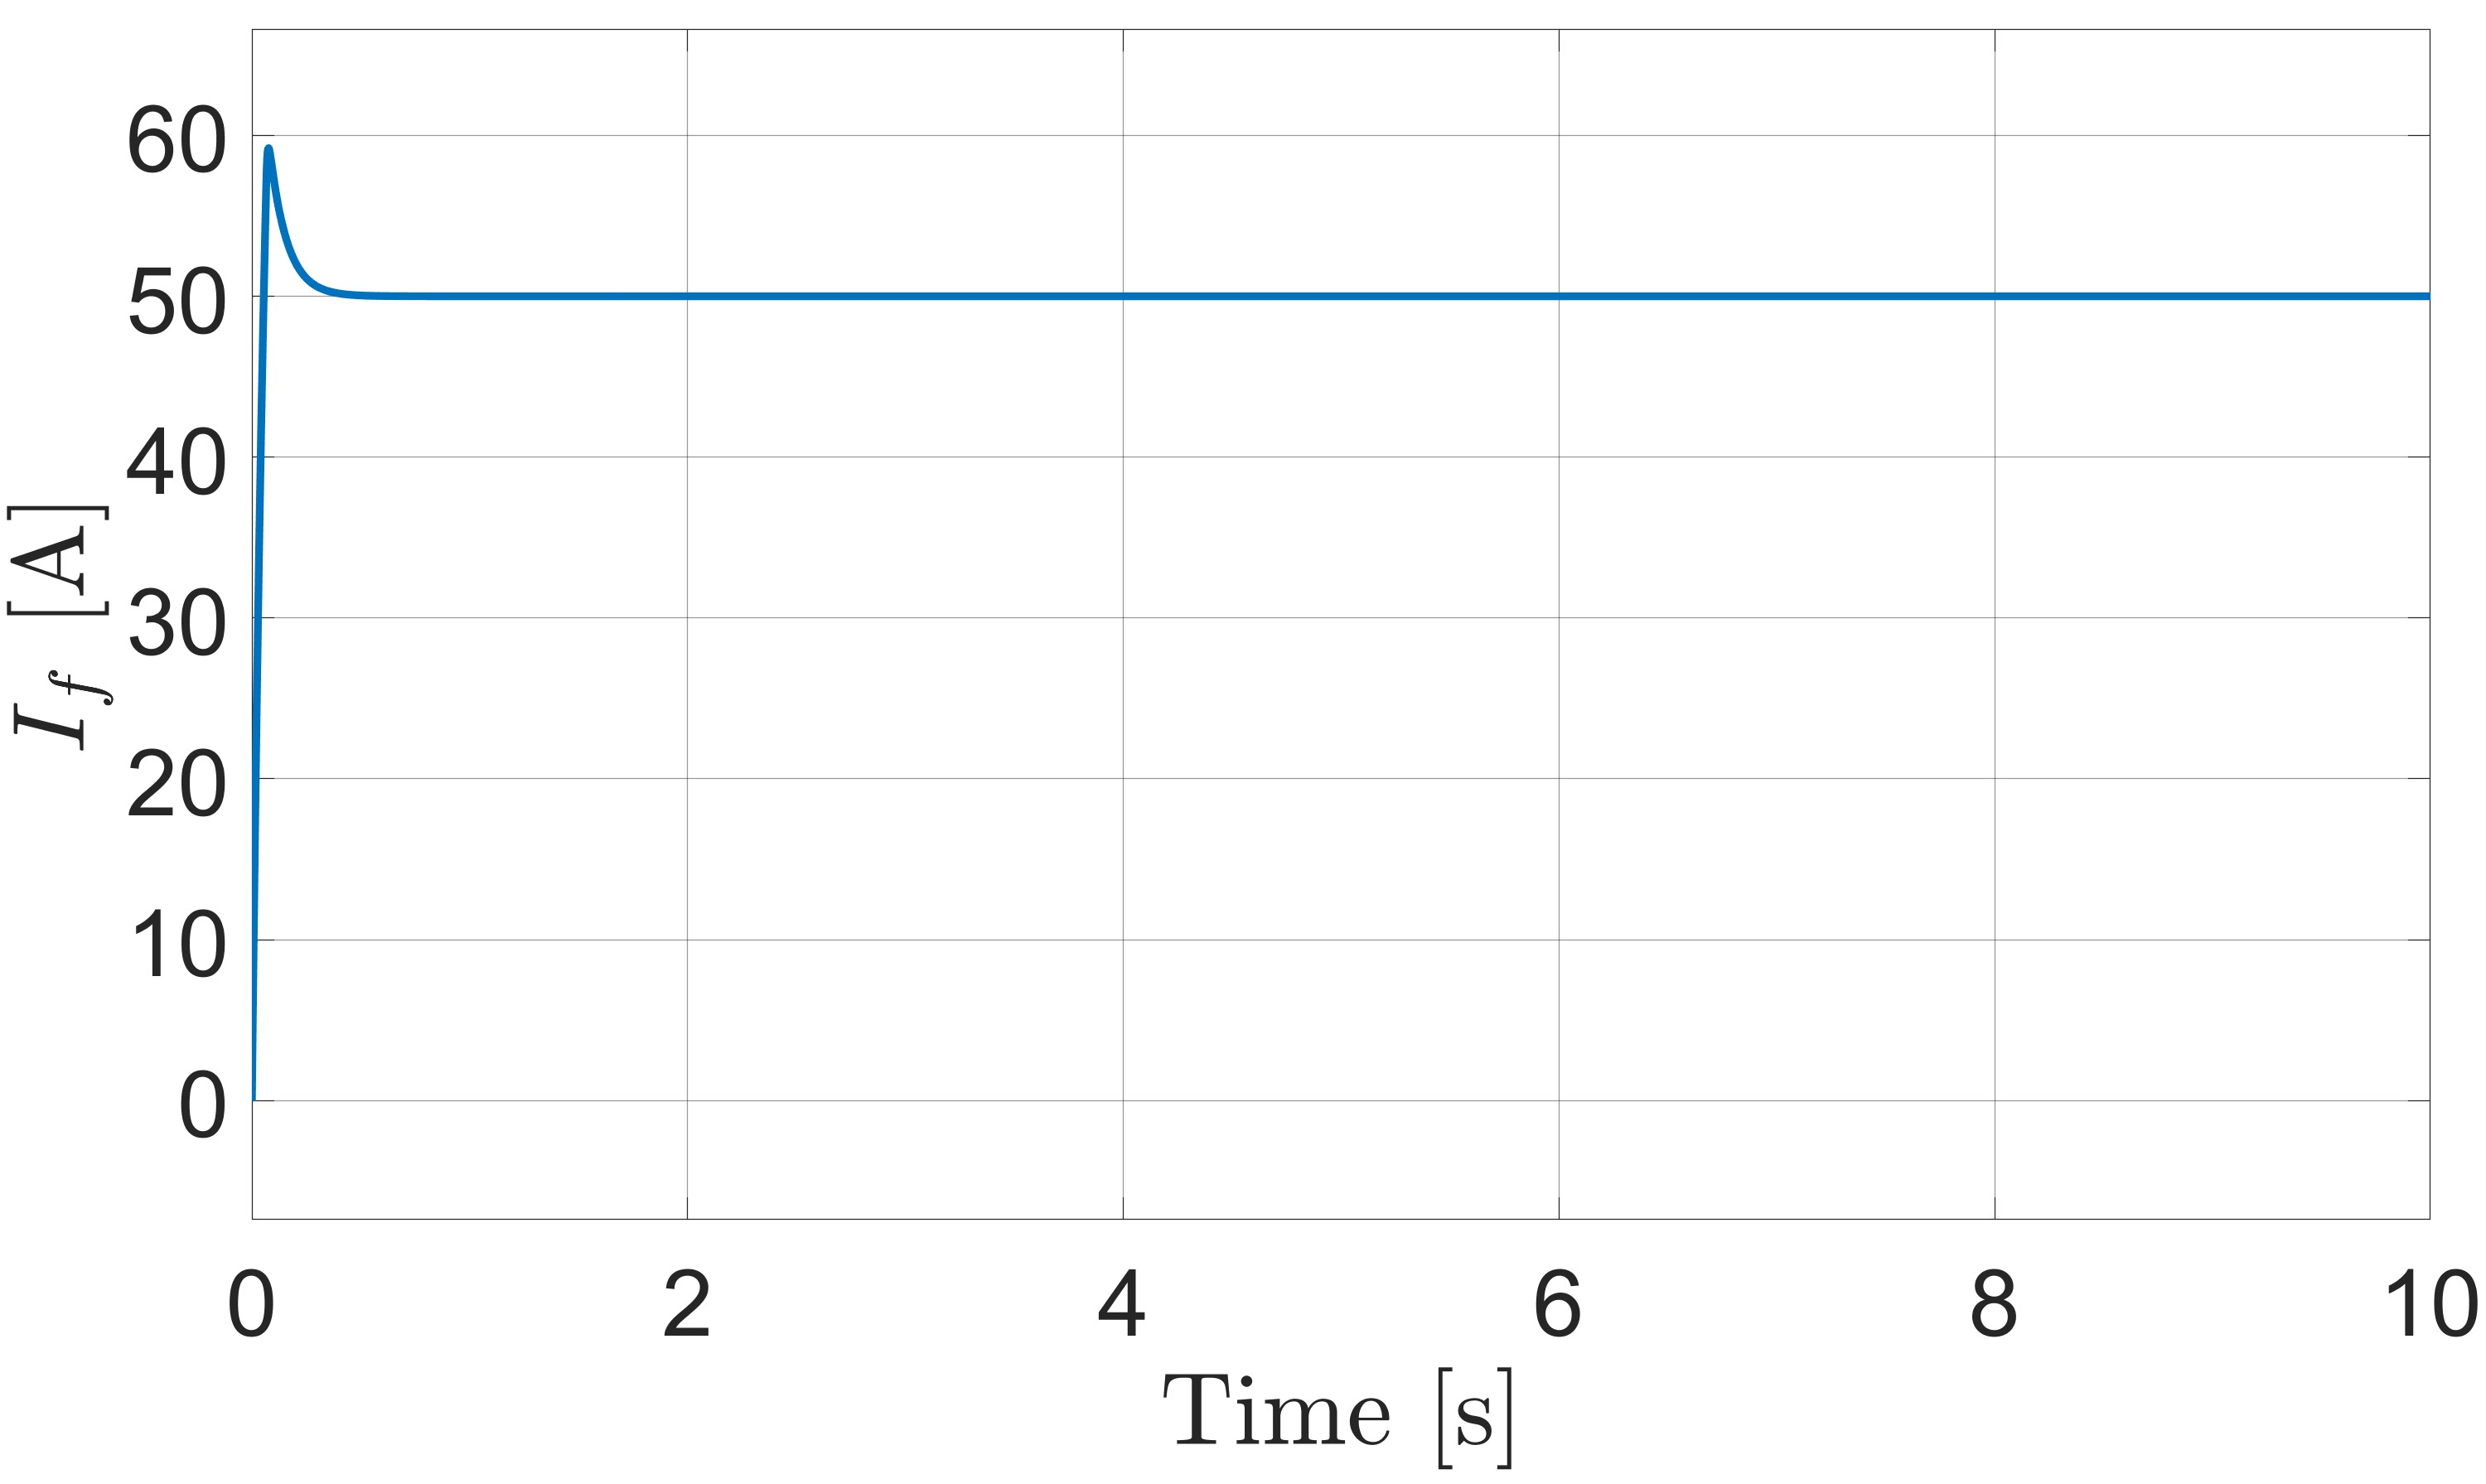
\includegraphics[width=0.6\linewidth]{PEMDT Exam Report/img/current response.jpg}
            \caption{Current response on start-up in derived transfer function}
            \label{fig: current resp}
        \end{figure}

    \subsection{Converter and Current Control Implementation}
        
        Comparing the derived transfer function to the provided machine on Figure \ref{fig: provided comparison} showed that at a settling time of 0.2s, the provided machine and the derived transfer function had a similar response; however, at a settling time of 0.4s, the derived transfer function still had an overshoot where-as the provided machine almost instantly settled with no overshoot. This difference is likely due to the converter and higher-order poles and zeros not being accounted for in the simplified transfer function. 
        \begin{figure}[tbh!]
            \centering
            \begin{subfigure}{0.44\textwidth}
                \centering
                 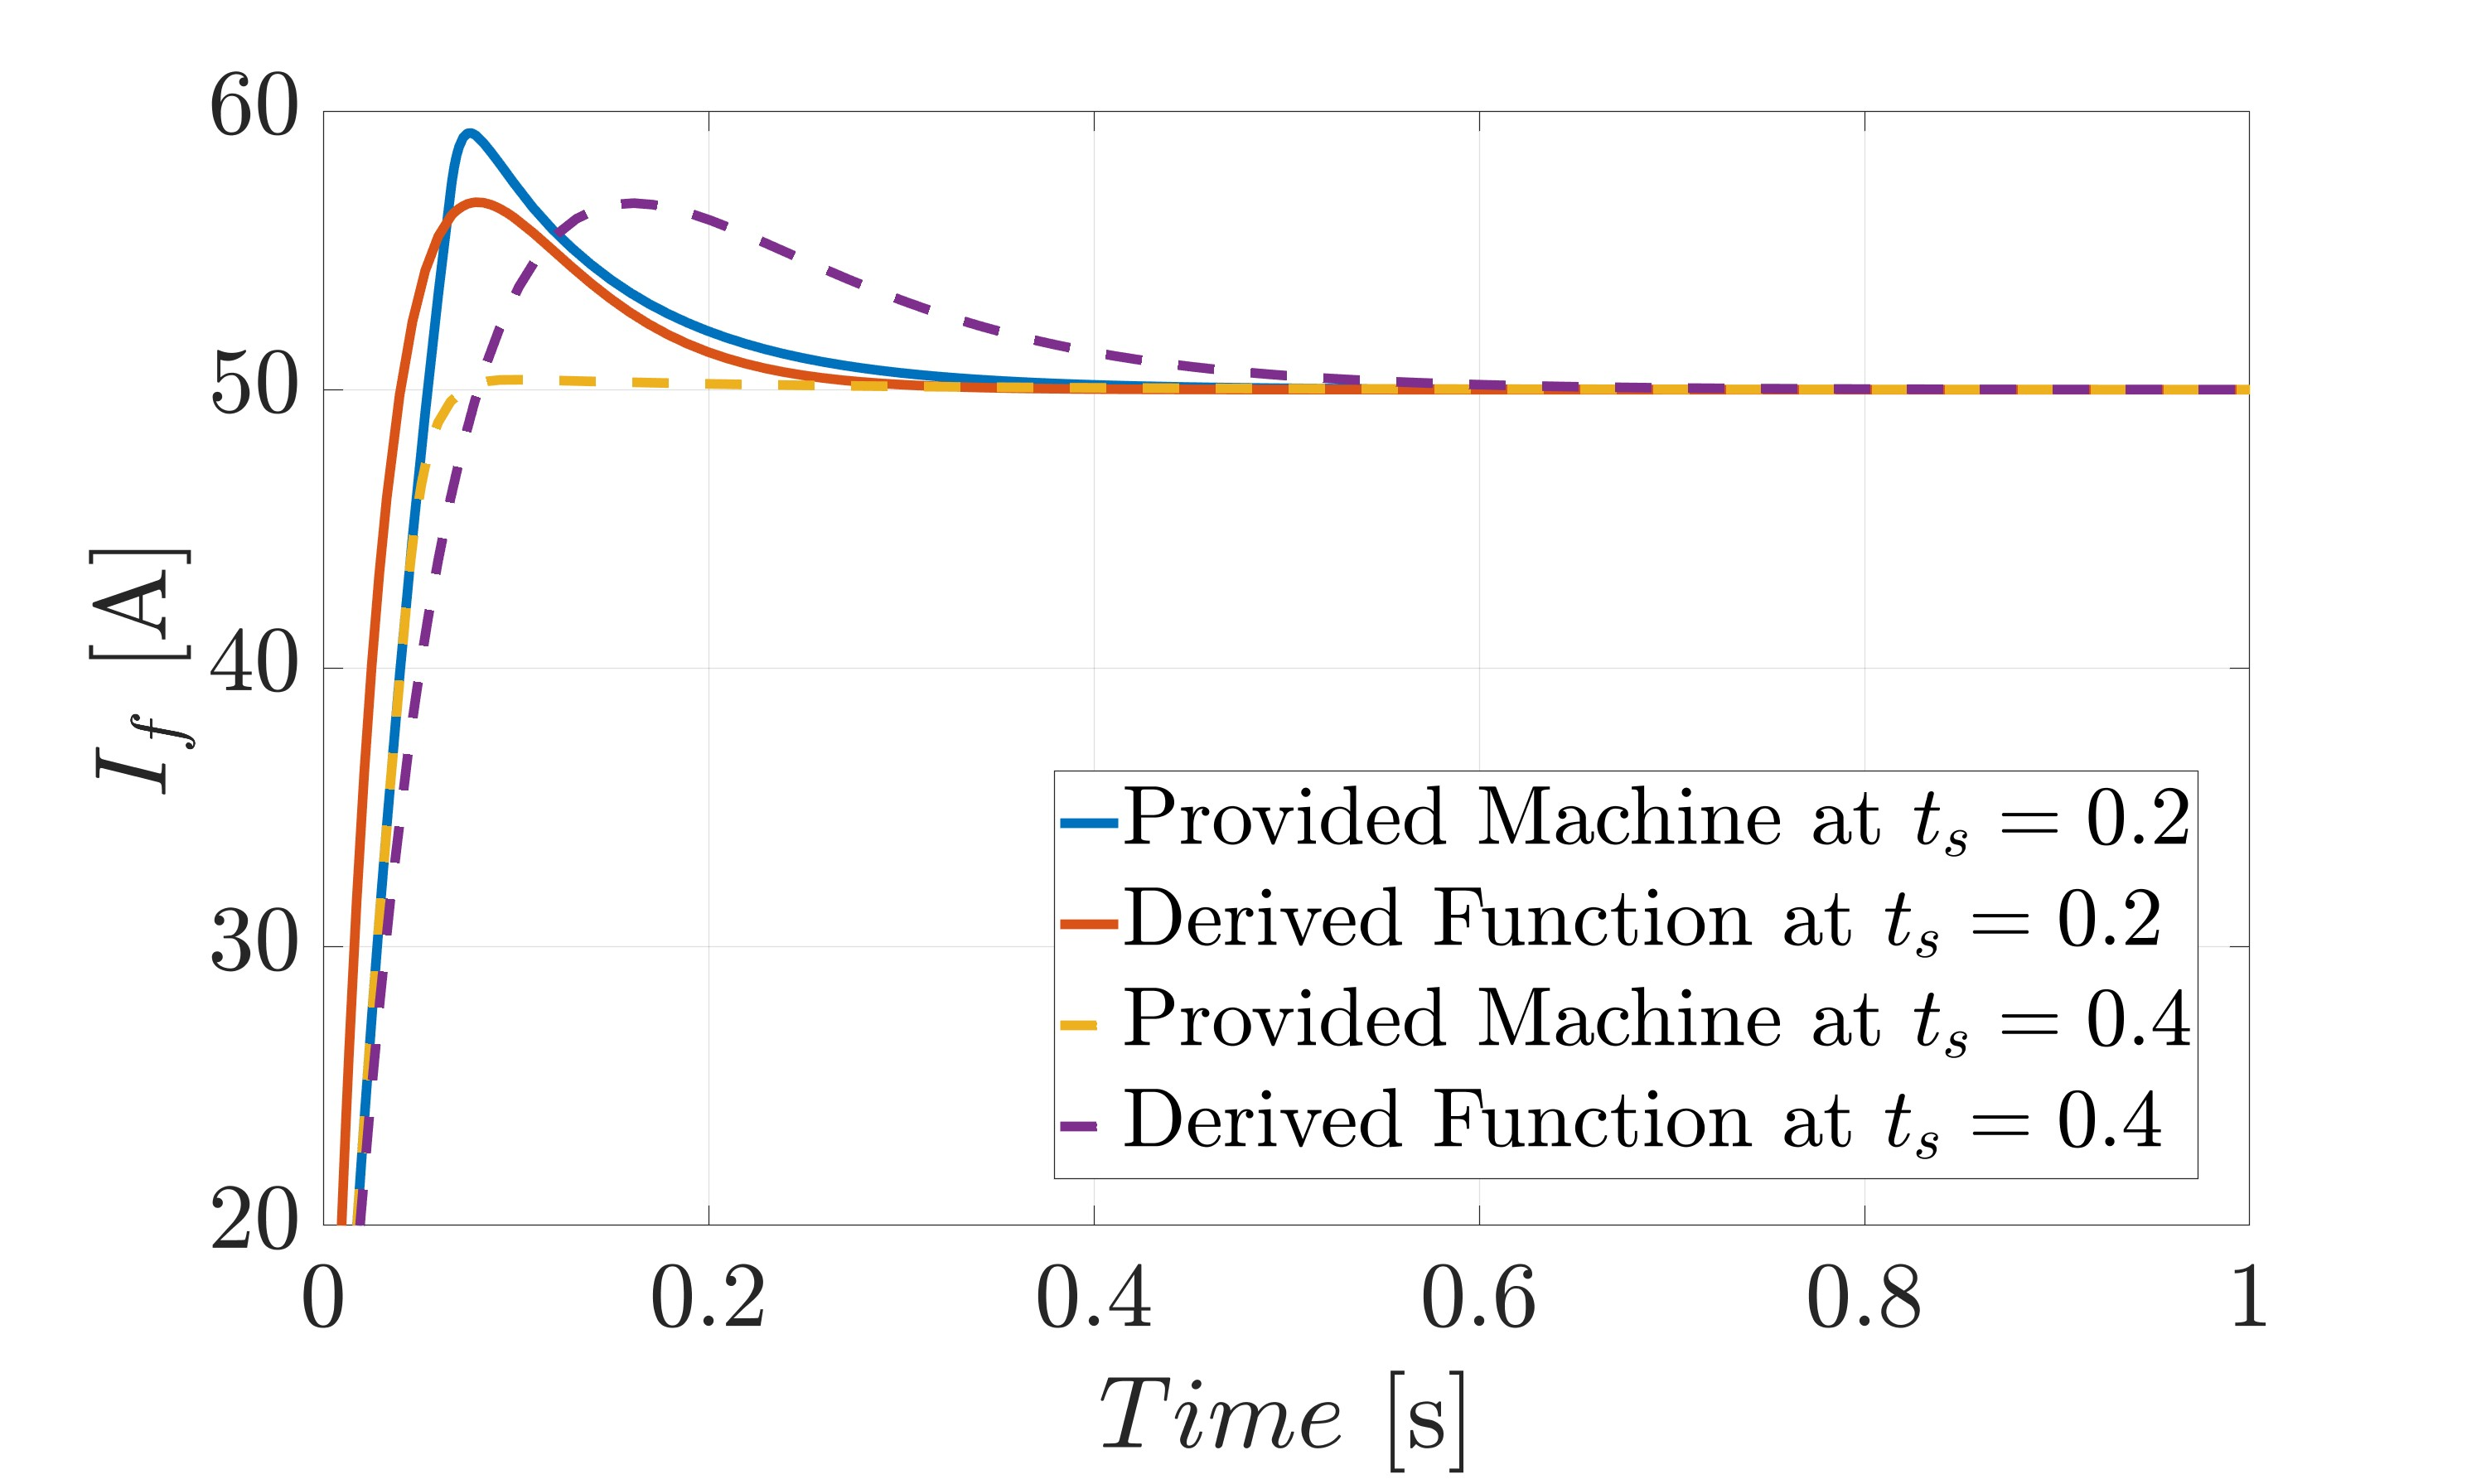
\includegraphics[width=\linewidth]{PEMDT Exam Report/img/Provided vs Derived current.jpg}
                 \caption{Current response in provided machine vs derived transfer function with same \(K_p\) and \(K_i\) values}
                 \label{fig: provided comparison}
            \end{subfigure}
            \hfill
            \begin{subfigure}{0.54\textwidth}
                 \centering
                 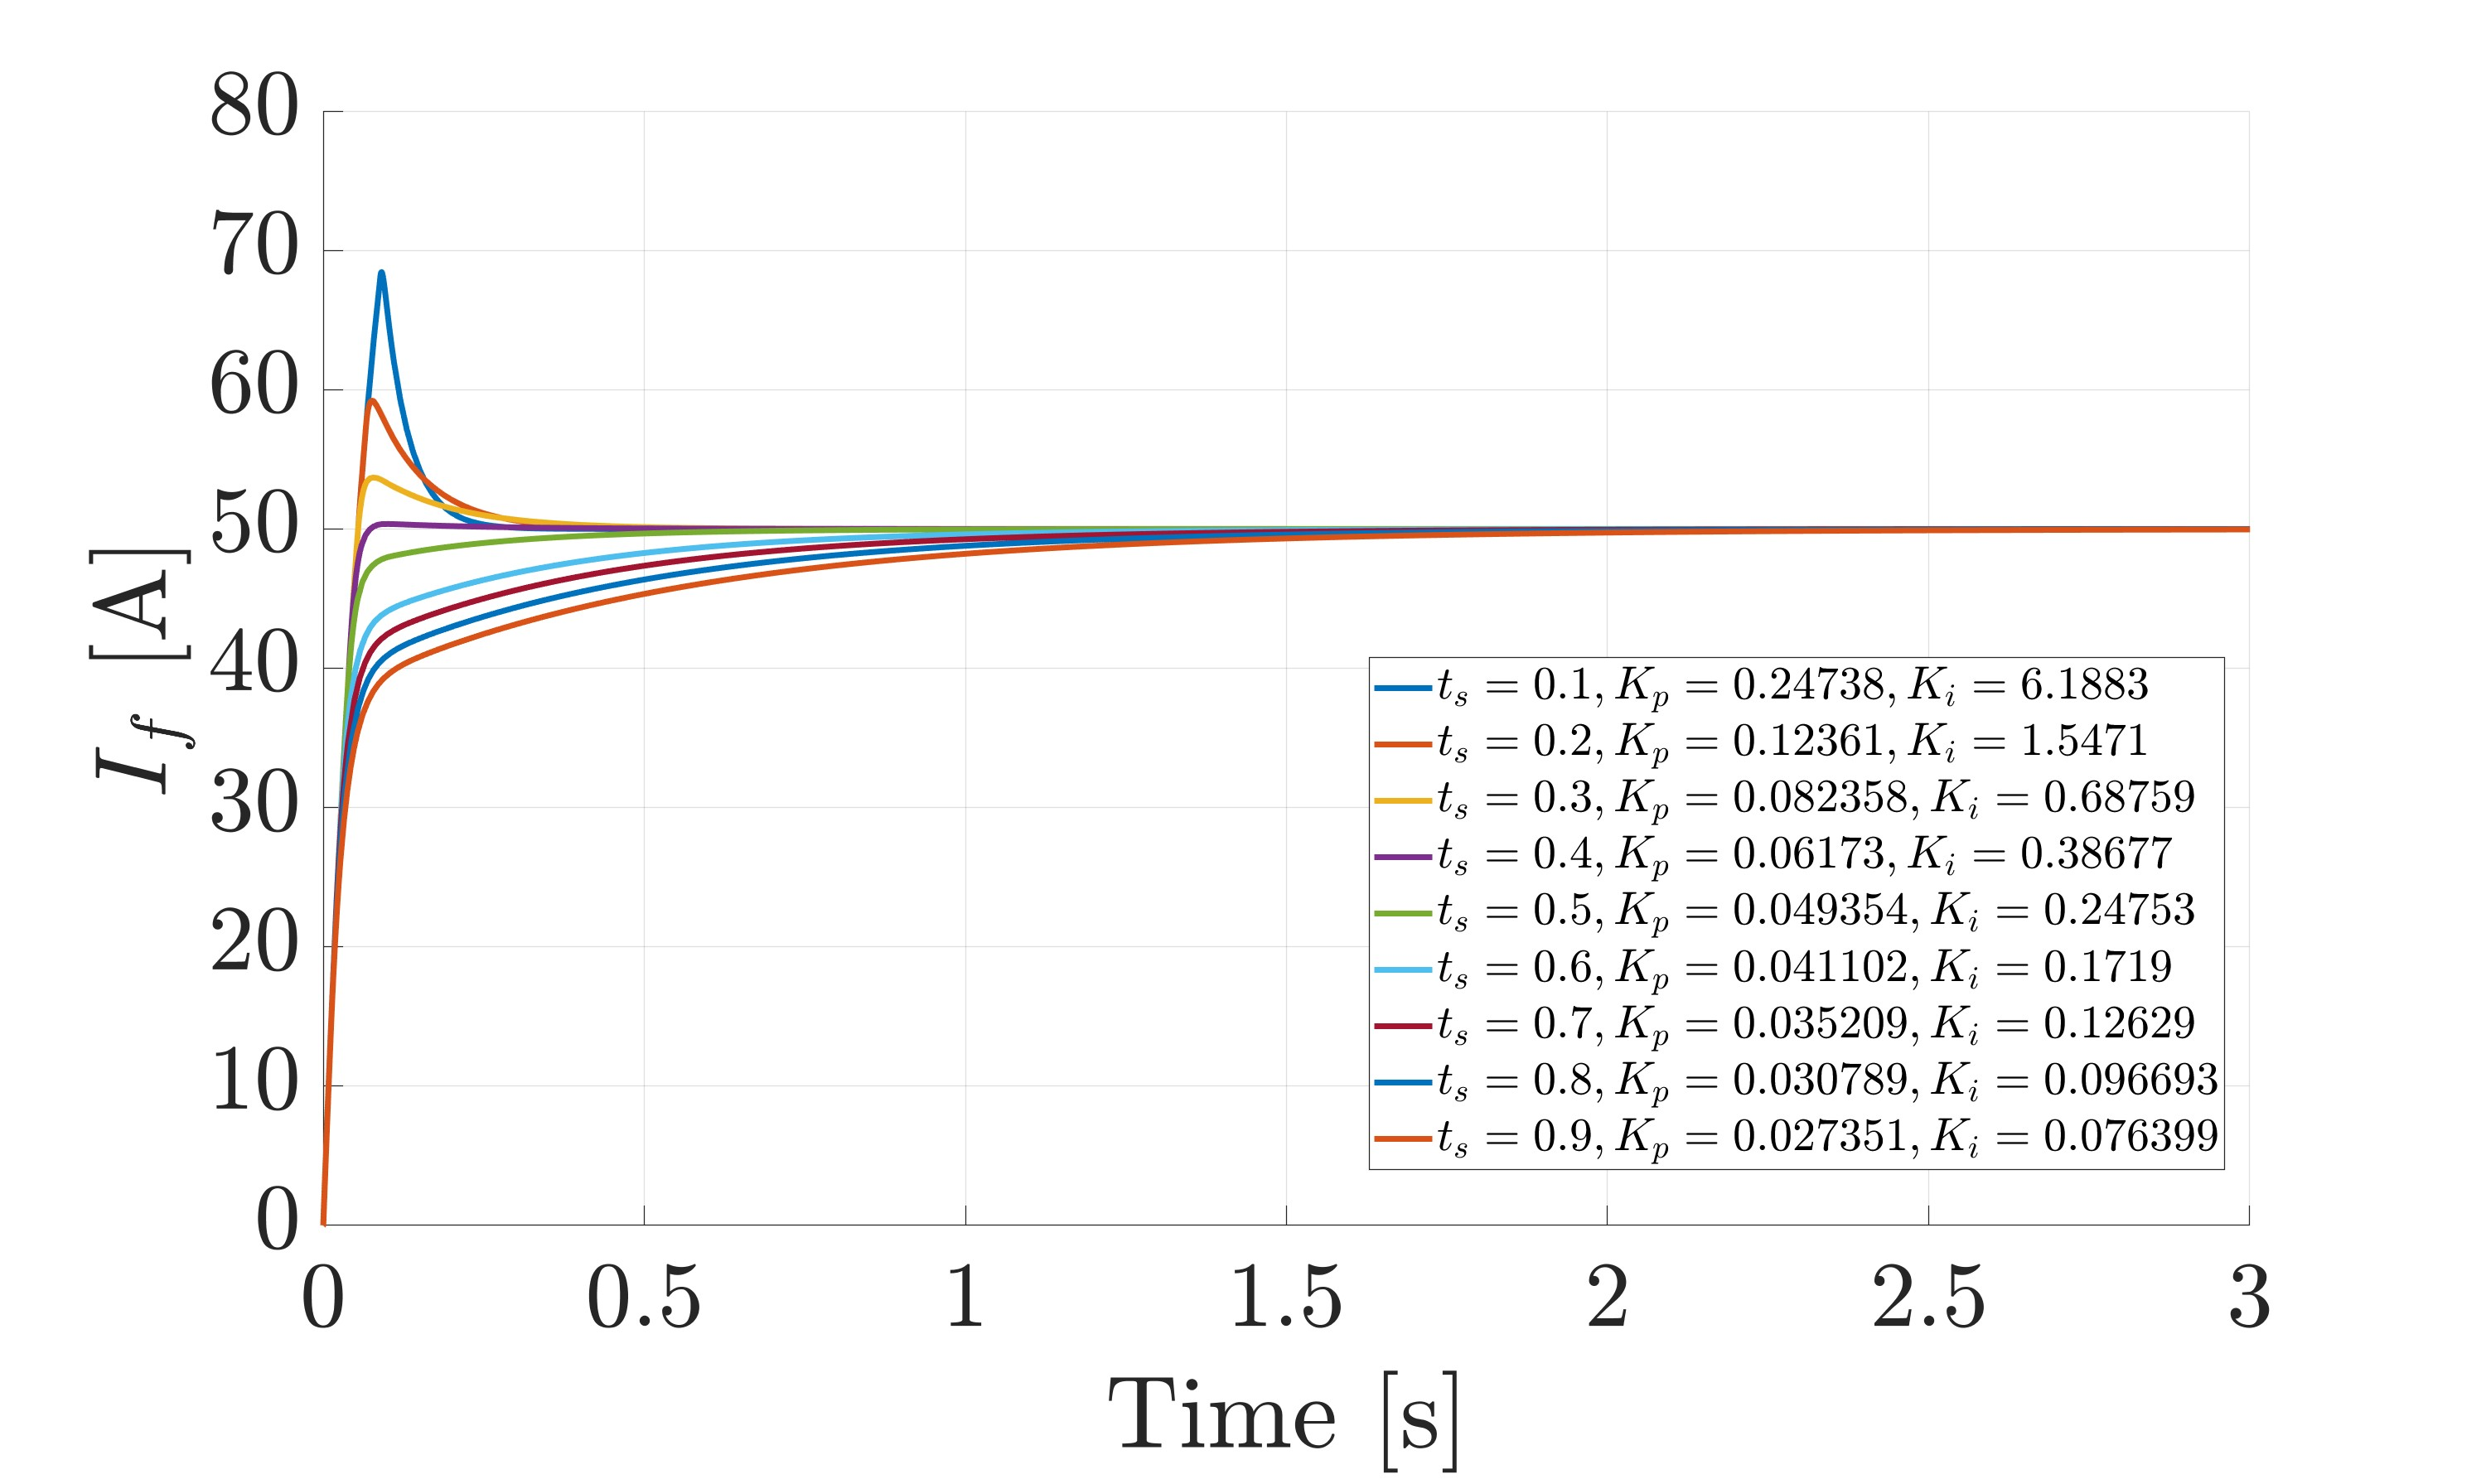
\includegraphics[width=\linewidth]{PEMDT Exam Report/img/Current settling time graph.jpg}
                 \caption{Testing different \(K_p\) and \(K_i\) values on the provided machine to tune values}
                 \label{fig: settling time test}
             \end{subfigure}
             \caption{Comparison of the derived transfer function to provided machine and fine-tuning on provided machine}
             \label{fig: comparison of current}
        \end{figure}
        With the provided machine behaving slightly differently, the \(K_p\) and \(K_i\) values were fine-tuned for the best response. As shown on Figure \ref{fig: settling time test} the best response was at \(\textbf{K}_\textbf{p} \textbf{= 0.062}\) and \(\textbf{K}_\textbf{i} \textbf{= 0.39}\).

    \subsection{Maximum Torque Limit}
        Given the system must not experience angular accelerations (\(\dot \omega\)) greater than 80 rad/s\(^2\), there will be a maximum torque that shouldn't be surpassed at specific rotational speeds (\(\omega\)). This was calculated using the following equations:
        \begin{align}
            T_{lim} &= \dot \omega J_{total} + \omega B_{total} \:\:\:\: &(\omega < 8000 \text{ rpm}) \\
            T_{lim} &= \dot \omega J_{total} + \omega B_{total} - 30 \:\:\:\: &(\omega \geq 8000 \text{ rpm})
        \end{align}
        where \(J_{total}\) and \(B_{total}\) are the systems mass moment of inertia and viscous friction terms, respectively. And the value of \(\omega\) in the calculation is in rad/s.

        The torque limit was graphed as shown in Figure \ref{fig: max torque}, and it was found that the instantaneous maximum torque that can be applied at the maximum angular acceleration is just before the turbofan is ignited at 8000 rpm and is 81.88 Nm.
        \begin{figure}[tbh!]
            \centering
            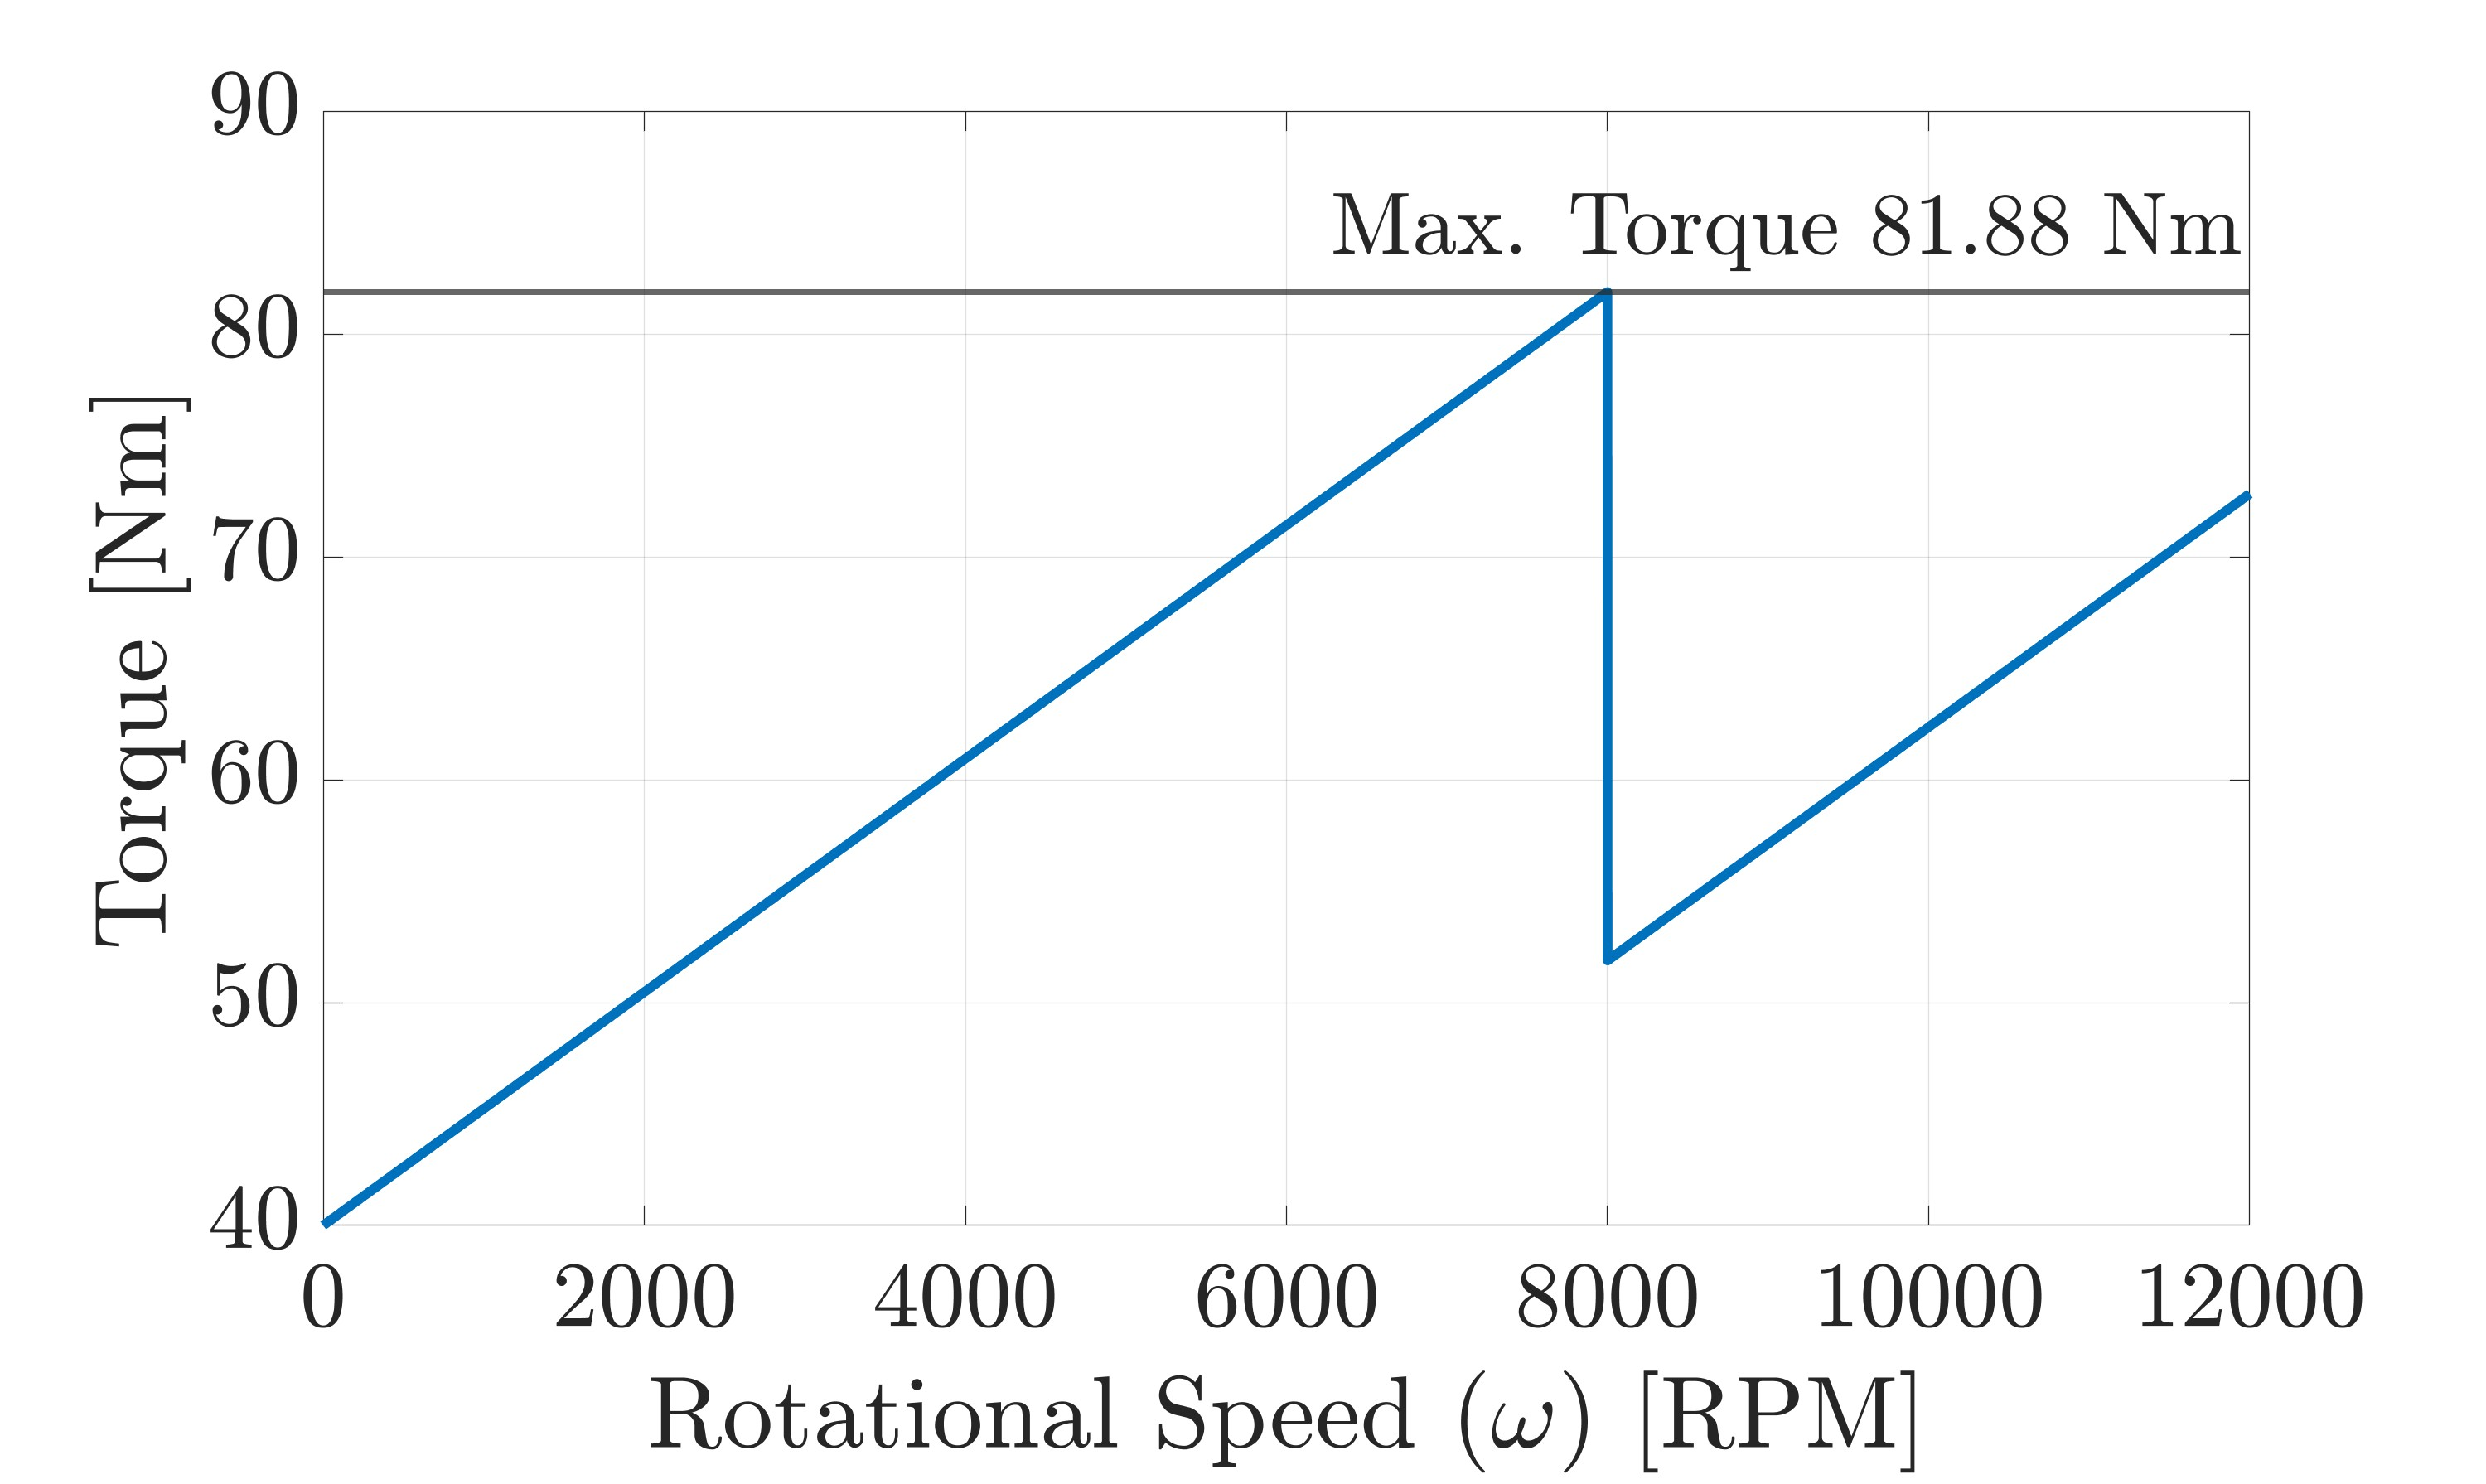
\includegraphics[width=0.6\linewidth]{PEMDT Exam Report/img/max torque.jpg}
            \caption{Max. torque limit under a max. angular acceleration of 80 rad/s\(^2\)}
            \label{fig: max torque}
        \end{figure}

    \subsection{Speed Controller Design}
        To design the speed controller, an equivalent transfer function of the speed loop was constructed. In order to construct this, it was assumed that only the Q axis generated torque, and the D axis affected the field. With this assumption, the closed loop transfer function being built was split into 3 parts: the control system (\(G_C^{\omega_R}\)), the current control loop (\(G_{CL}^{i_a}\)) and the machine control loop (\(G_M^{\omega_R}\)). These were all combined into one transfer function to obtain the closed-loop speed control using the following equation:
        \begin{align}
            G_{CL}^{\omega_R} = \frac{G_C^{\omega_R}(s) G_{CL}^{i_a}(s) G_M^{\omega_R}(s)}{1 + G_C^{\omega_R}(s) G_{CL}^{i_a}(s) G_M^{\omega_R}(s)} \label{speed loop}
        \end{align}
        Where:
        \begin{align}
            G_C^{\omega_R}(s) = \frac{K_p^\omega}{s}\left(s+\frac{K_i^\omega}{K_p^\omega}\right) && G_M^{\omega_R}(s) = \frac{\frac{1}{J_{total}}}{s+\frac{B_{total}}{J_{total}}}
        \end{align}
        Equation (\ref{speed loop}) includes the closed-loop current control system; however, it has been assumed that the control system being modelled has a bandwidth an order of 10 times smaller than the control circuit, and therefore, it is assumed that the current controller doesn't have such a large effect on the transfer function and is just a unity gain (\(G_{CL}^{i_a}(s) = 1\)). The equation for the closed-loop speed control loop can now be written as:
        \begin{align}
            G_{CL}^{\omega_R} = \frac{G_C^{\omega_R}(s) G_M^{\omega_R}(s)}{1 + G_C^{\omega_R}(s) G_M^{\omega_R}(s)} = \frac{\frac{K_p^\omega}{J_{total}}\left(s + \frac{K_i}{K_p}\right)}{s^2 + s\left(\frac{B_{total}+K_p^\omega}{J}\right) + \frac{K_i^\omega}{J_{total}}}
        \end{align}
        As for the current controller designed previously, the characteristic equation of this transfer function was compared to an ideal system that is critically damped (shown in Eq. (\ref{ideal sys})). In this instance, the settling time (\(t_s\)) was set to 30\% of the 120s threshold, and it is said to be 5 times larger than the time period \(T\). This produced the following values for \(K_p^\omega\) and \(K_i^\omega\):
        \begin{align}
            K_p^\omega = \frac{2J_total}{T} - B_{total} = 0.117 && K_i^\omega = \frac{J_{total}}{T^2} = 0.0139
        \end{align}
        A similar transfer function was created for the case where a load is applied. Its transfer function was given as follows:
        \begin{align}
             G_{CL}^{\omega_R} = \frac{\frac{K_p^\omega}{J_{total}}\left(s + \frac{K_i}{K_p}\right)}{s^2 + s\left(\frac{B_{total}+K_p^\omega}{J} + \frac{T_{load}}{\omega_{avg}J_{total}}\right) + \frac{K_i^\omega}{J_{total}}}
        \end{align}
        Which, at a load of 10 Nm and an average rotational speed of 100 rad/s change \(K_p^\omega\) to the following:
        \begin{align}
            K_p^\omega = \frac{2J_total}{T} - B_{total} - \frac{T_{load}}{\omega_{avg}J_{total}} = 0.0167
        \end{align}
        \begin{figure}[tbh!]
            \centering
            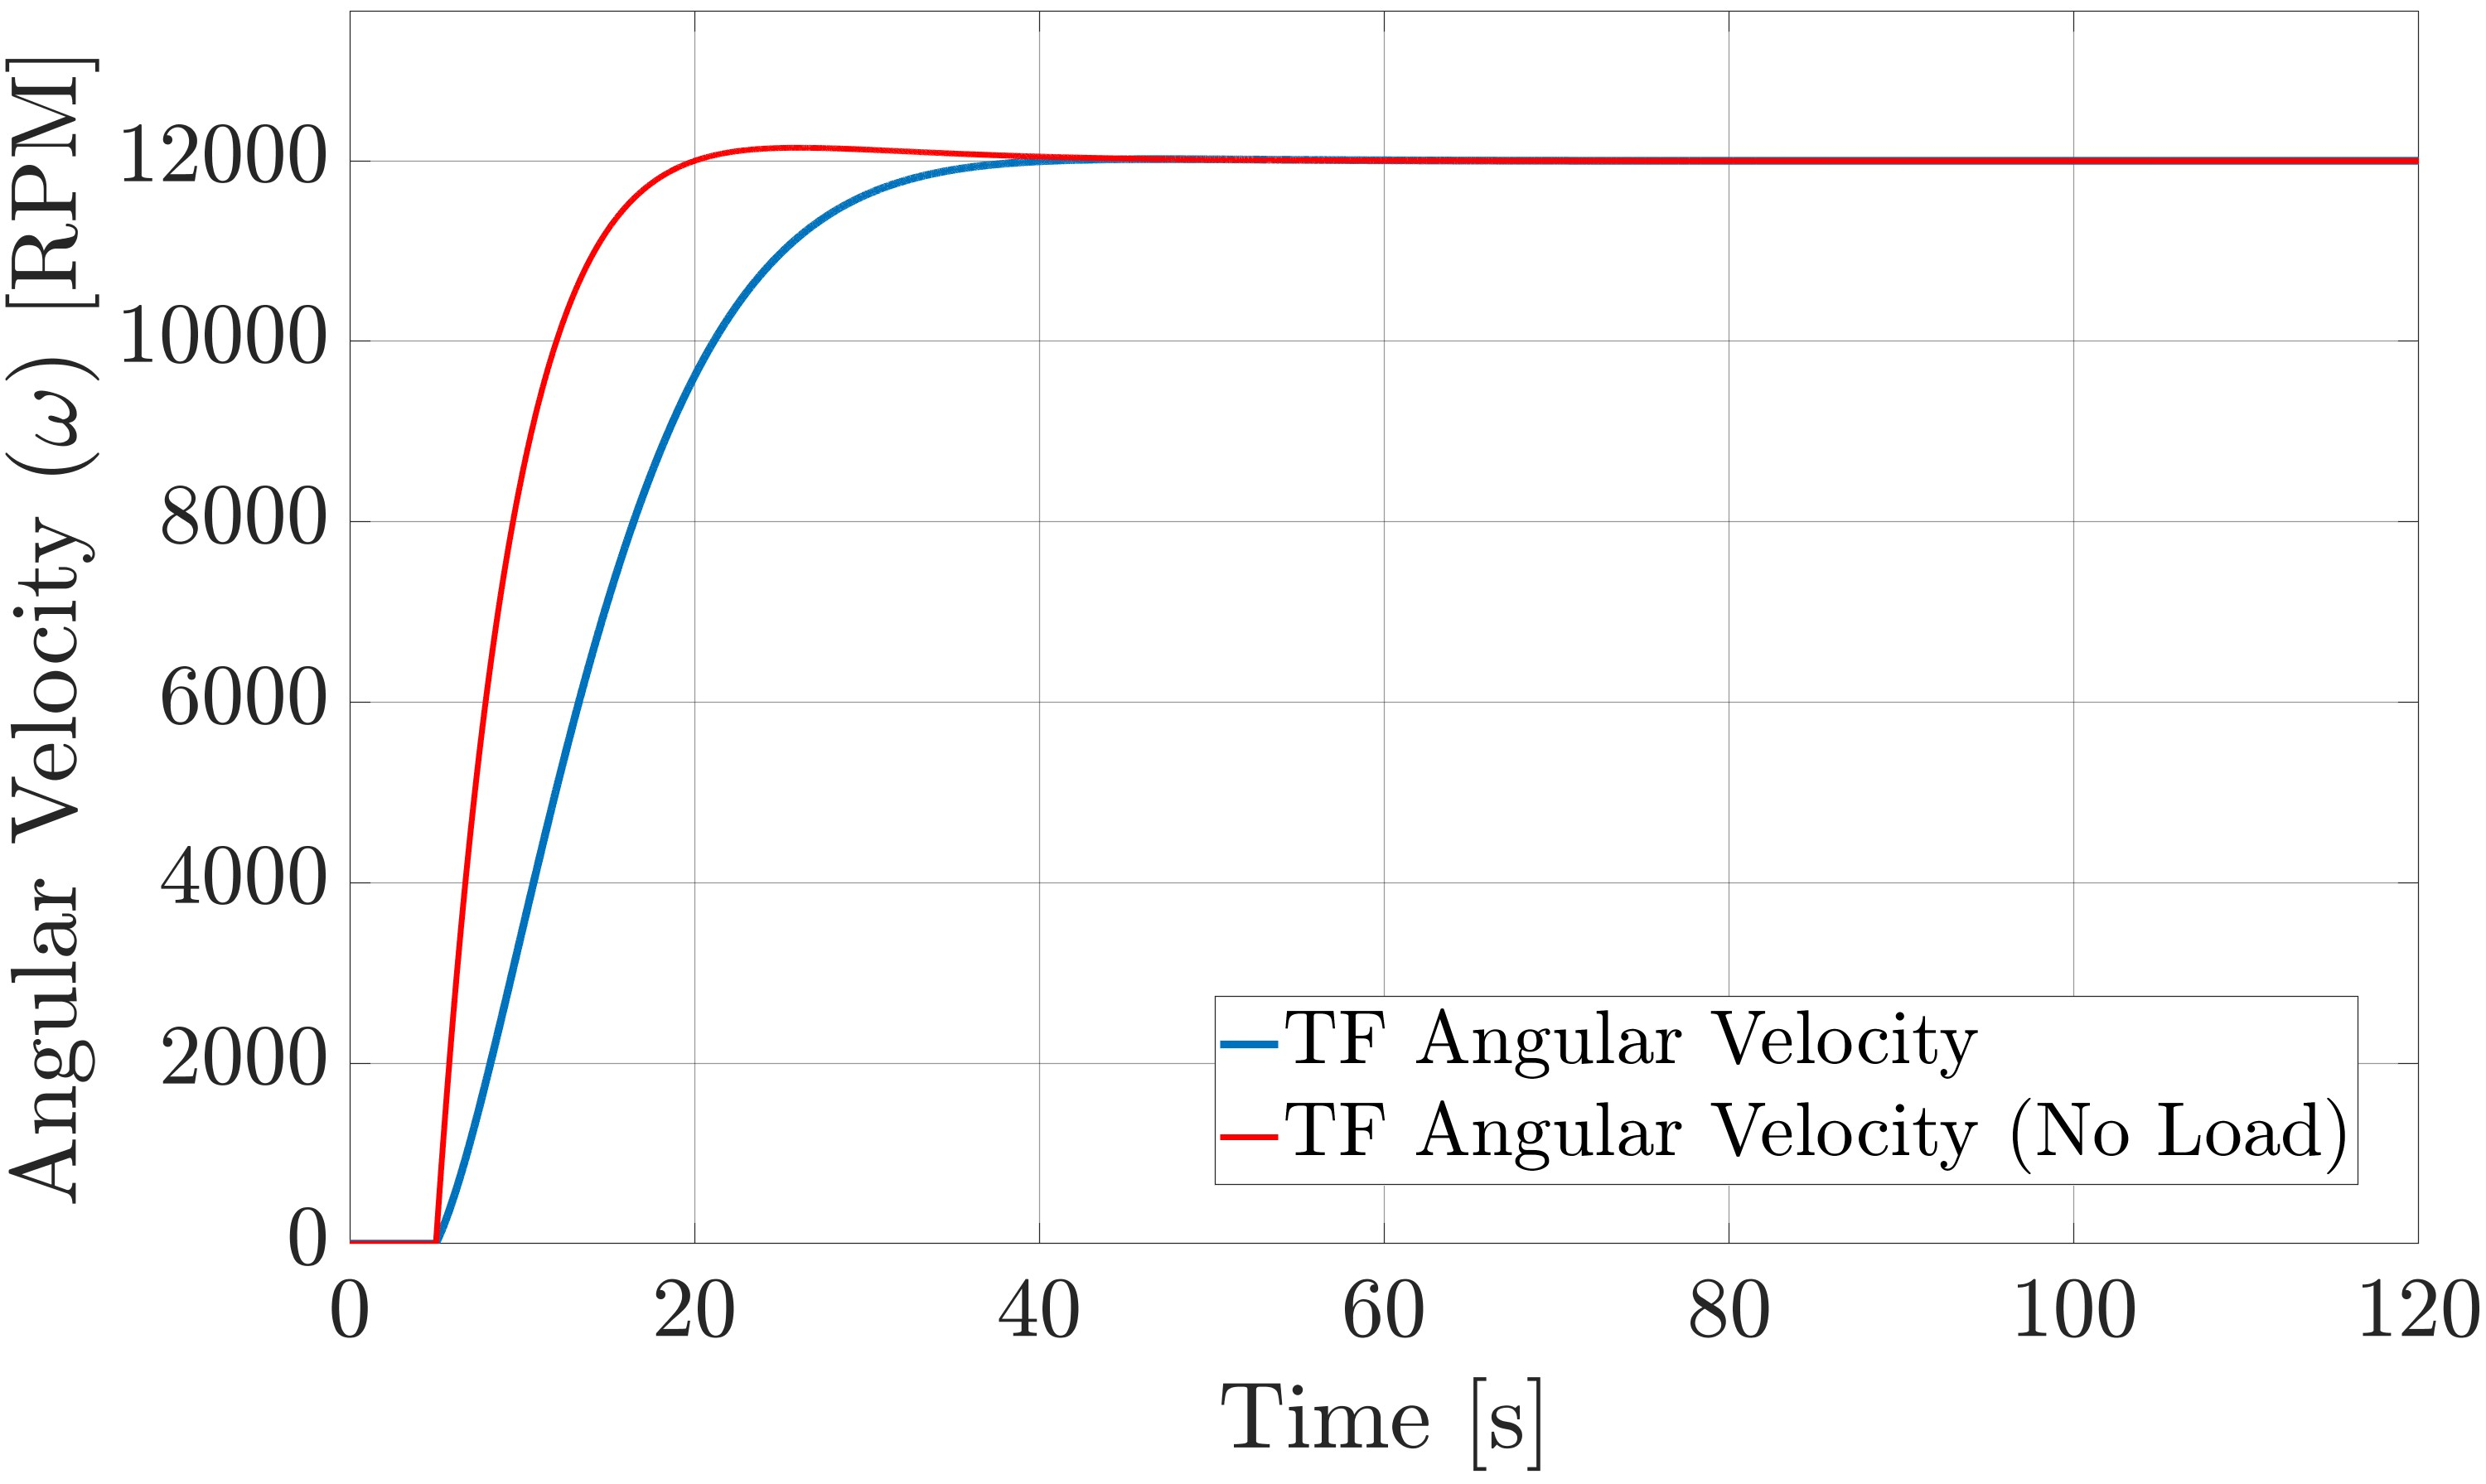
\includegraphics[width=0.6\linewidth]{PEMDT Exam Report/img/Speed Control TF.jpg}
            \caption{Response of speed control transfer function with and without a load at a 30s settling time}
            \label{fig: speed control tf}
        \end{figure}
        Figure \ref{fig: speed control tf} shows that the transfer function definitely achieves two out of the three criteria, settling at 12,000 RPM and having as close to a non-oscillatory response as possible. The acceleration threshold required more complex dynamics, which proved difficult to model with the given resources.

    \subsection{Speed Control Implementation}